\documentclass[aip,jap,reprint,amsmath,amssymb]{revtex4-2}
\usepackage{graphicx}
\usepackage{booktabs}
\usepackage[hidelinks]{hyperref}

\begin{document}

\title{Can equilibrium excitonic-insulator switches beat CMOS? A benchmarked feasibility screen across the BEC--BCS crossover}

\author{Nailah Masyhur}
\email{nailahmasyhur@gmail.com}
\affiliation{Department of Physics, Faculty of Mathematics and Natural Sciences, Universitas Indonesia, Depok 16424, Indonesia}

\date{\today}

\begin{abstract}
Exciton condensates and excitonic insulators have been proposed as switches that operate below the
$\ln(10)k_BT/e \approx 60$~mV/decade thermionic limit of complementary metal-oxide-semiconductor (CMOS)
transistors, which would reduce the energy cost of computing. We test this premise for gate-driven devices in
thermal equilibrium, using mean-field models with Gaussian fluctuations in which every ingredient is first benchmarked against a published result:
a two-dimensional (2D) electron--hole gap equation across the BEC--BCS crossover; self-consistent
screening in the superfluid state, validated against diffusion quantum Monte Carlo (DQMC); massless Dirac
bands for graphene double layers; a quasi-one-dimensional three-chain model of Ta$_2$NiSe$_5$ with
exciton--phonon coupling; Gaussian order-parameter fluctuations; gate electrostatics; and
Abrikosov--Gor'kov disorder. Screening together with the Nelson--Kosterlitz bound gives a ceiling
$T_c \le \mathrm{Ry}^*/4r_{s,c}^2$, where $r_{s,c}(d/a_B)$ is the density at which the superfluid appears.
No hBN-encapsulated double layer reaches 300~K. For monolayer-graphene double layers at the operating point of the
bilayer pseudospin field-effect transistor, the gap vanishes under both normal-state and superfluid-state
screening. In Ta$_2$NiSe$_5$ the ordered state is mostly excitonic ($\approx$70--77\%) but requires the lattice, and its
discrete symmetry breaking precludes superfluidity. The only sub-CMOS switching found, an abrupt
mean-field gap onset, does not survive Gaussian fluctuations: the swing becomes 100--470~mV/decade at
300--350~K, rising to $\ge$285~mV/decade once gate electrostatics are included. Switching energy at equal
geometry is therefore 2--45 times higher than ideal CMOS. A machine-learning surrogate trained on the
benchmarked physics finds no buildable design above $\approx$120~K with hBN dielectrics. These results identify
2D phase stiffness under screening, rather than pairing, as the bottleneck for equilibrium excitonic low-power logic.
Tunnelling-based and non-equilibrium switching mechanisms lie outside this screen.
\end{abstract}

\maketitle

\section{Introduction}

Electricity use by data centres is projected to roughly double between 2024 and 2030, with artificial
intelligence as the main driver~\cite{IEA2025}. A fundamental limit on the energy per logic operation in
CMOS is the subthreshold swing $S \ge \ln(10)k_BT/e$, which sets the minimum gate voltage per decade of
current, 60~mV/decade at room temperature~\cite{IonescuRiel2011}. Devices that sidestep this
``Boltzmann tyranny'' are actively sought.

Excitonic systems have been proposed in this context. An excitonic insulator (EI) forms when the
single-particle gap $E_g$ is smaller than the exciton binding energy $E_b$, and the ground state is a
BCS-like condensate of electron--hole pairs~\cite{Jerome1967,Kaneko2013}. In bilayers with spatially separated
electrons and holes~\cite{LozovikYudson1976,Pieri2007} the condensate supports counterflow superfluidity~\cite{LozovikYudson1976,Min2008}. On this basis the
bilayer pseudospin field-effect transistor (BiSFET) was proposed, with a simulated switching energy of
0.008~aJ per clock cycle, compared with $\sim$5~aJ for end-of-roadmap CMOS~\cite{Banerjee2009}.
Its key assumption is a room-temperature condensate in graphene double layers, based on an unscreened
mean-field estimate $T\sim 0.1E_F$~\cite{Min2008}. Including carrier screening lowers this estimate by many
orders of magnitude~\cite{Kharitonov2008}. Experimentally, signatures of excitonic order exist in
Ta$_2$NiSe$_5$~\cite{Wakisaka2009,Lu2017,Seki2014}, 1$T$-TiSe$_2$~\cite{Kogar2017},
monolayer WTe$_2$~\cite{Jia2022,Sun2022}, TMD double layers~\cite{Wang2019,Ma2021},
InAs/GaSb~\cite{Du2017} and graphene double bilayers in the quantum Hall regime~\cite{Li2017,Liu2017}.
Room-temperature excitonic transistors exist, but they operate without a condensate~\cite{Unuchek2018}.

This work asks a narrow question. Given the pairing physics as understood in the literature, can an
excitonic switch beat CMOS at chip temperatures (300--350~K)? The approach is a chain of models in which
each ingredient reproduces a published number before it is used (Table~\ref{tab:bench}), so the
conclusion does not rest on unvalidated approximations. All code is openly available~\cite{repo}.

\section{Models and methods}

\subsection{2D continuum gap equation}
Electrons and holes with reduced mass $m_r$ pair through
$V(q)=2\pi e^2 e^{-qd}/[\epsilon q(1+r_0q)]$, with layer separation $d$, background dielectric constant
$\epsilon$ and Rytova--Keldysh length $r_0$~\cite{Berkelbach2013}. The gap equation is
\begin{equation}
\begin{aligned}
\Delta_k&=\sum_{k'}V_{kk'}\frac{\Delta_{k'}}{2E_{k'}}\tanh\frac{E_{k'}}{2k_BT},\\
E_k&=\sqrt{\xi_k^2+\Delta_k^2},\qquad \xi_k=\frac{E_g}{2}+\frac{\hbar^2k^2}{4m_r},
\end{aligned}
\label{eq:gap}
\end{equation}
where $\mu_{\rm eff}=-E_g/2$ plays the role of the chemical potential in the BEC--BCS crossover~\cite{Randeria2014}.
The radial Nystr\"om discretisation uses an analytic angular integral (complete elliptic integrals) and
cell-averaging of the integrable logarithmic singularity. In 2D the mean-field $T^*$ is only a pairing scale on the
BEC side~\cite{Randeria2014}. The condensation temperature is bounded by the Nelson--Kosterlitz
jump~\cite{NelsonKosterlitz1977}, $k_BT_{\rm BKT}\le \pi\hbar^2 n_s/2M$ with $M=m_e+m_h$ and $n_s\le n$.

\subsection{Screening in the superfluid state}
At fixed pair density $n$ [effective units $a_B^*$ and $\mathrm{Ry}^*$; $r_s=(\pi n)^{-1/2}/a_B^*$; one species per layer~\cite{Pieri2007}],
the pairing interaction is screened by the carriers of the paired state [superfluid-state (SS) screening]~\cite{Neilson2014}:
\begin{equation}
V^{\rm SS}_q=\frac{v_q e^{-qd}}{1+2v_q\Pi(q)+[v_q\Pi(q)]^2(1-e^{-2qd})},
\label{eq:ss}
\end{equation}
with $v_q=2\pi e^2/\epsilon q$,
and $\Pi=\Pi_n+\Pi_a$ is built from BCS coherence factors,
$\Pi(q)=\sum_k(u_kv_{k'}-v_ku_{k'})^2/(E_k+E_{k'})$ with $k'=k+q$. It reduces to the static 2D Lindhard function for $\Delta\to0$ and
vanishes as $q\to0$ in the superfluid. Iteration starts from the unscreened (US) coherent state. Neilson \textit{et al.} showed that this SS approach, unlike US or normal-state (NS) screening, reproduces the DQMC condensate fraction~\cite{Neilson2014}.

\subsection{Dirac bands}
For graphene double layers we use the two-band Dirac model~\cite{Min2008}, $\xi_k=\hbar vk-E_F$, coupling $\alpha=e^2/\epsilon\hbar v$, chirality factor
$(1+\cos\theta)/2=[(k+k')^2-q^2]/4kk'$ and four spin--valley copies. Three screening treatments are compared:
US~\cite{Min2008}; NS random-phase approximation~\cite{Kharitonov2008}; and SS screening
as in Eq.~(\ref{eq:ss}), with the intraband polarisability from coherence factors and the interband part kept at its
normal-state value.

\subsection{Quasi-1D chains: Ta$_2$NiSe$_5$}
We use the three-chain Hubbard model of Kaneko \textit{et al.}~\cite{Kaneko2013}. It has two Ta $5d$ conduction chains and one
Ni--Se valence chain, with $t_c=-0.8$, $t_f=0.4$ and $D=0.2$~eV fitted to density-functional theory. It includes on-site $U$, interchain
$V=U/4$, and a uniform shear phonon with $\lambda=g^2/\omega$. Since the mean-field equations of
Ref.~\onlinecite{Kaneko2013} are given in supplementary material, we derive them from its Hamiltonian:
Hartree terms for $U$ and $V$, Fock terms on both c--f bonds, a static $q=0$ phonon, and opposite order on the
two Ta chains.

\subsection{Fluctuations, gate and disorder}
Gaussian fluctuations are included through a Ginzburg--Landau expansion of the Gibbs--Bogoliubov variational
free energy along the mean-field pair shape, with stiffness $\hbar^2/2M$. The quartic term is treated in the
self-consistent Hartree (large-$N$) approximation~\cite{UllahDorsey1991,LarkinVarlamov2005} with Bose occupation of
the pair modes, $\langle|\psi|^2\rangle=\sum_Q n_B(a+b\langle|\psi|^2\rangle+cQ^2)$. Gaussian fluctuations
about the normal state are equivalent to the Nozi\`eres--Schmitt-Rink scheme~\cite{NozieresSchmittRink1985,Randeria2014}.
The fluctuation-broadened gap follows the pseudogap form $\Delta^2=\Delta_{\rm sc}^2+\Delta_{\rm pg}^2$~\cite{Chen2005}.
Gate electrostatics follow Ref.~\onlinecite{Zeng2020}: $e\,dV=(C+d\mu_x/dn)\,dn$ with
$C=4\pi e^2d_s/\epsilon$. A thermal compressibility term $k_BT/n$ is added because the pair gas is non-degenerate at 300~K.
Disorder enters through the Abrikosov--Gor'kov equation as applied to bilayers~\cite{Bistritzer2008}.

\subsection{Device metrics}
For a gap-switching transistor we assume intrinsic activated conduction, $G\propto e^{-E_{\rm gap}/2k_BT}$~\cite{Sze2007}. The swing is then
$S=2\ln(10)k_BT/|dE_{\rm gap}/d(eV)|$, which is compared with $S_{\rm CMOS}=\ln(10)k_BT/e$. This is an idealised off-state. It ignores
sub-gap states and contact resistance, both of which would increase $S$, and band-to-band tunnelling, which is a distinct mechanism not
evaluated here. The mean-field overestimate of $T_c$ by $(4e)^{1/3}\approx2.2$ was derived for weak-coupling contact interactions in
three dimensions~\cite{GorkovMB1961,Randeria2014}. Here it is used only as a heuristic robustness check on whether pairing survives at the
operating temperature. The conclusions of Sec.~\ref{sec:switch} hold without it, because the fluctuation analysis removes the sub-CMOS
swing independently.
For the BiSFET, the criterion is a 2D condensate at the operating temperature. Switching energy at equal geometry scales
as $(S_{\rm EI}/S_{\rm CMOS})^2$. As a sanity check, $C_gWLV^2$ for the BiSFET geometry gives 0.0044~aJ, against the
SPICE value of 0.008~aJ~\cite{Banerjee2009}.

\begin{table*}
\caption{Benchmarks reproduced before each ingredient is used; all rows are regenerated by \texttt{run\_benchmarks.py}~\cite{repo}. Literature values read from figures are approximate ($\approx\pm0.03$). Two Ta$_2$NiSe$_5$ rows are documented deviations (see text).}
\label{tab:bench}
\begin{ruledtabular}
\begin{tabular}{llll}
ingredient & quantity & literature & this work\\
\hline
2D gap equation & 2D exciton $E_b=4\,\mathrm{Ry}^*$ & 435.4 meV (exact) & 432.9 meV\\
 & EI exists only for $E_g<E_b$ & Ref.~\onlinecite{Jerome1967} & yes\\
crossover mean field & 3D unitarity $\Delta/E_F$, $\mu/E_F$ & 0.68, 0.59~\cite{Randeria2014} & 0.686, 0.591\\
 & BCS-limit $T_c$ & $(8\gamma/\pi e^2)E_Fe^{-\pi/2k_F|a|}$~\cite{Randeria2014} & within 1\%\\
fixed-density bilayer & $\Delta_{\max}$ at $d=a_B$, $r_s=1.5,3,20$ & 0.66, 0.68, 0.18 Ry*~\cite{Pieri2007} & 0.659, 0.700, 0.173\\
SS screening & superfluid onset $r_{s,c}$, $d=a_B$ & 2.5 (DQMC), $\approx3$ (SS)~\cite{Neilson2014} & 2.38\\
 & onset, $d=0.7a_B$ & 2.1 (DQMC)~\cite{Neilson2014} & 1.97\\
Dirac, NS screening & $V_{\rm us}(p_F)/V(p_F)$, $\alpha=1$ & $\approx9$~\cite{Kharitonov2008} & 8.99\\
 & $\lambda_c^{\max}$ & 1/16~\cite{Kharitonov2008} & 0.0624\\
 & $d\lambda/d\ln(1/T)$ vs.\ $\lambda_c$ ($\alpha=1$) & equal~\cite{Kharitonov2008} & 0.0546 vs.\ 0.0567\\
Ta$_2$NiSe$_5$ chains & distortion onset $\lambda_c$ & 0.125 eV~\cite{Kaneko2013} & 0.125 eV\\
 & EI onset $V_c$ & 0.6 eV~\cite{Kaneko2013} & 0.69 eV (+15\%)\\
 & $k_BT_c$ ($V=0.55$, $\lambda=0.04$ eV) & 0.0783 eV~\cite{Kaneko2013} & 0.0564 eV ($-$28\%)\\
gate & interlayer $E_b$, $d=a_B$ & 0.77 Ry* (linear fit)~\cite{Zeng2020} & 0.866 Ry* (exact)\\
disorder & $dT_c/d\delta$; critical $\delta$ & $-\pi/4$; 0.88$T_{c0}$~\cite{Bistritzer2008} & $-0.7855$; 0.8819$T_{c0}$\\
energy & BiSFET switching energy & 0.008 aJ~\cite{Banerjee2009} & 0.0044 aJ ($CV^2$)\\
\end{tabular}
\end{ruledtabular}
\end{table*}

\section{Results}

\subsection{Crossover and the pairing--condensation gap}
Figure~\ref{fig:crossover} shows the 2D crossover for MoSe$_2$/hBN/WSe$_2$-like parameters ($m_r=0.22$,
$\epsilon=4.5$, $d=1.6$~nm). On the BCS side, $\Delta_k$ peaks at the Fermi wavevector and $v_k^2$ has a Fermi edge. On the BEC side, both are
smooth. With the unscreened interaction, the mean-field pairing scale $T^*$ exceeds 350~K over most of the EI window, but the BKT bound keeps
the condensation temperature below $\approx$200~K, and at only tens of kelvin near the crossover. Screening (Sec.~\ref{sec:ceiling}) removes the high-density end. This separation of $T^*$ and $T_c$ on the BEC side mirrors the cold-atom
phase diagram~\cite{Randeria2014}. It is the first sign that the bottleneck is phase stiffness, not pairing.

\begin{figure*}
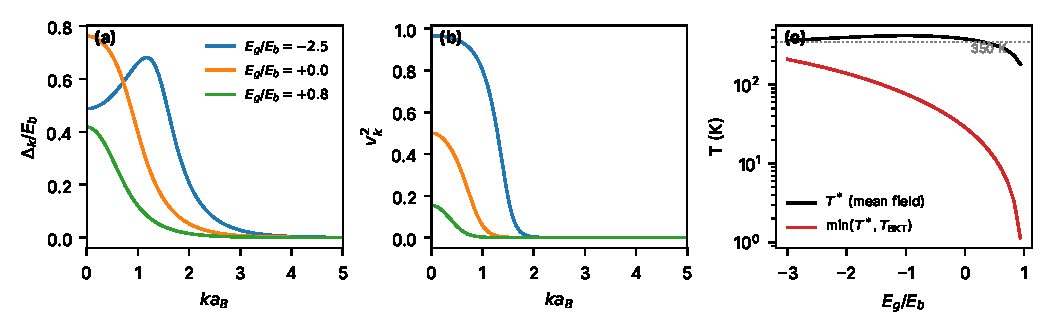
\includegraphics[width=\textwidth]{figs/fig1_crossover.pdf}
\caption{BEC--BCS crossover in a 2D e--h double layer with the unscreened interaction ($m_r=0.22$, $\epsilon=4.5$, $d=1.6$~nm; representative MoSe$_2$/hBN/WSe$_2$ values). (a) Gap function, (b) pair
occupation, (c) mean-field pairing scale $T^*$ and condensation estimate $\min(T^*,T_{\rm BKT})$ versus $E_g/E_b$.}
\label{fig:crossover}
\end{figure*}

\subsection{Screening ceiling}\label{sec:ceiling}
With superfluid-state screening, a large-gap superfluid exists only for $r_s>r_{s,c}(d/a_B)$, in agreement
with diffusion quantum Monte Carlo [Fig.~\ref{fig:ceiling}(a)]. Below $r_{s,c}$, screening suppresses the
gap exponentially~\cite{Neilson2014}. Combining this with $n_s\le n$ gives
\begin{equation}
k_BT_c\le \frac{\mathrm{Ry}^*}{4r_{s,c}^2}\,\frac{4m_r}{m_e+m_h},
\label{eq:ceiling}
\end{equation}
where equal masses is the most favourable case. With the MoSe$_2$/WSe$_2$ parameters of Ref.~\onlinecite{Zeng2020} ($m_r\approx0.2$, $\epsilon\approx5$, $d=a_B\approx1.3$~nm) the bound is 57~K. With the representative values used in Figs.~\ref{fig:crossover} and~\ref{fig:switch} ($m_r=0.22$, $\epsilon=4.5$, $d=1.6$~nm) it is 49~K, and at the thinnest barrier, $d=0.7$~nm, it is 112--121~K. Across $0.05\le m_r\le0.6$, $2\le\epsilon\le15$ and $0.6\le d\le3$~nm, no point
reaches 350~K, and none with $\epsilon\ge4.5$ reaches 300~K [Fig.~\ref{fig:ceiling}(b)]. The maximum is 328~K, reached at $\epsilon=2$. This result is unchanged when $r_{s,c}$ is extrapolated linearly below the smallest computed separation, $d/a_B=0.3$. Valley and spin
degeneracy add screening channels and lower the bound further.

\begin{figure*}
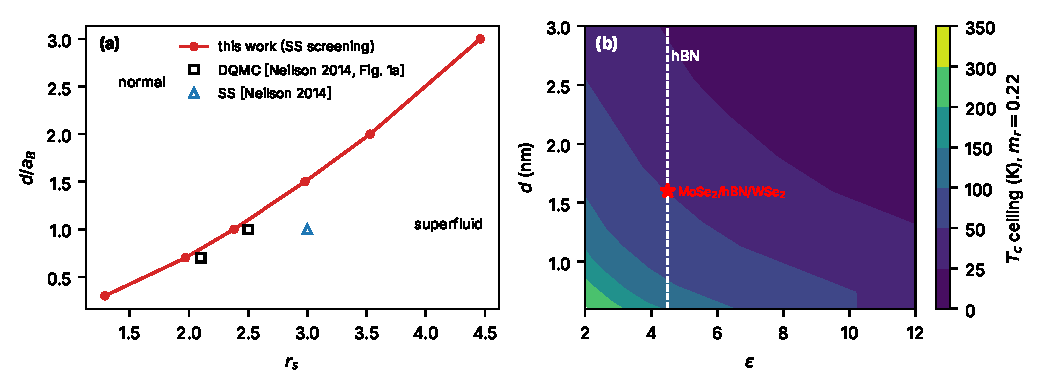
\includegraphics[width=\textwidth]{figs/fig2_screening_ceiling.pdf}
\caption{(a) Superfluid onset $r_{s,c}$ versus layer separation with superfluid-state screening, compared with DQMC and
mean-field SS points read from Ref.~\onlinecite{Neilson2014}. (b) Screening ceiling, Eq.~(\ref{eq:ceiling}), for
$m_r=0.22$. The white contour marks 300~K and the dashed line marks hBN ($\epsilon=4.5$).}
\label{fig:ceiling}
\end{figure*}

\subsection{Graphene double layers: the BiSFET operating point}
At the BiSFET density ($n=4.9\times10^{12}$~cm$^{-2}$, $E_F=258$~meV), with $d=1$~nm and $\epsilon=3.9$, the unscreened
Dirac gap is $\Delta=31$~meV ($\approx0.12E_F$), consistent with Ref.~\onlinecite{Min2008}. This
corresponds to $T_{\rm KT}\le E_F/8\approx374$~K. With normal-state screening the coupling is
$\lambda_c<1/16$ and $T_c\sim10^{-7}E_F$~\cite{Kharitonov2008}. With superfluid-state screening the gap collapses
within two iterations. Even at $\epsilon=1$ and $d=0.3$~nm it converges to 0.087~meV. Monolayer-graphene double layers therefore
do not condense at useful temperatures under either screening treatment validated in the literature. This agrees with
the conclusion of Ref.~\onlinecite{Neilson2014} for monolayer graphene at 1~nm separation.

\subsection{Ta$_2$NiSe$_5$}
In the three-chain model (Fig.~\ref{fig:tns}) the order is cooperative. At $V=0.55$~eV, below the purely excitonic threshold, order appears only for $0.02<\lambda<0.04$~eV or larger. For $\lambda=0.04$--0.05~eV, 69--74\% of the c--f hybridisation is excitonic, and 77\% with the alternative decoupling discussed below. A purely
structural instability would need $\lambda\ge0.125$~eV, 2.5--6 times the estimate $\lambda\approx0.02$--0.05~eV inferred from the measured
distortion~\cite{Kaneko2013}. Our implementation reproduces the published distortion threshold exactly, but it places the purely excitonic threshold 15\% higher ($V_c=0.69$ vs.\ 0.6~eV) and $k_BT_c$ 28\% lower than Ref.~\onlinecite{Kaneko2013} (Table~\ref{tab:bench}). Two alternative Fock decouplings bracket both published values, so the deviation reflects mean-field decoupling details given in that work's supplementary material. The thresholds are therefore sensitive to the decoupling at the 15--30\% level, whereas the excitonic share of the order is not: it stays at 74--77\% across decouplings at $V=0.55$~eV, $\lambda=0.04$~eV. We therefore claim only that the order is predominantly excitonic, not a precise ratio. The device conclusion for Ta$_2$NiSe$_5$ below rests on the symmetry analysis of Ref.~\onlinecite{Mazza2020}, not on these numbers. The mean-field $T_c$ divided by 2.2 gives 298--377~K, which brackets the measured
326~K~\cite{Lu2017}. Symmetry analysis based on first-principles Wannier models shows that the transition
breaks only discrete symmetries and that there is no excitonic superfluidity~\cite{Mazza2020}. This is consistent with the early observation that interband transitions in a homogeneous excitonic insulator fix the phase of the order parameter and make superfluidity impossible~\cite{LozovikYudson1976}. The structural
interpretation of Ref.~\onlinecite{Baldini2023} is compatible with our finding that the lattice decides
whether order sets in. For devices, Ta$_2$NiSe$_5$ cannot host a counterflow condensate, and as a bulk crystal its gap can
be tuned only by pressure or strain.

\begin{figure}
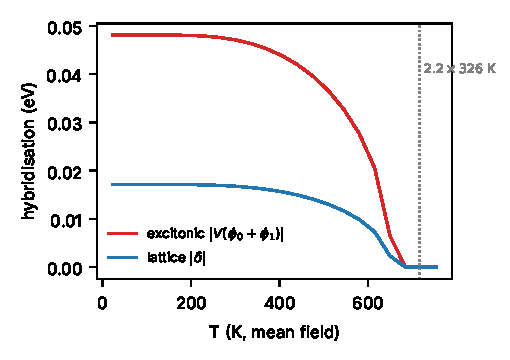
\includegraphics[width=\columnwidth]{figs/fig4_ta2nise5.pdf}
\caption{Ta$_2$NiSe$_5$ three-chain model~\cite{Kaneko2013} at $V=0.55$~eV, $\lambda=0.04$~eV: excitonic and lattice
contributions to the c--f hybridisation versus mean-field temperature.}
\label{fig:tns}
\end{figure}

\subsection{Switching steepness and energy}\label{sec:switch}
The only sub-CMOS swing found in mean field comes from an abrupt gap onset where $T^*(E_g)$ crosses the
operating temperature: 60.4~mV/decade at 350~K for MoSe$_2$/hBN/WSe$_2$ and 38.6~mV/decade at 300~K for WTe$_2$
(Fig.~\ref{fig:switch}). Gaussian fluctuations replace this onset with a smooth pseudogap crossover, giving
$S=102$--140 and 137--280~mV/decade respectively across a factor-of-four range of momentum cut-off. The
Ginzburg--Landau quartic reproduces the mean-field amplitude to within 4\%. A real gate makes the situation
worse. At 300~K, interlayer charging plus the thermal compressibility of the pair gas give $S\ge285$~mV/decade.
A negative exchange compressibility~\cite{Zeng2020} alone would give 49~mV/decade, but this gain does not survive
at non-degenerate densities. At equal geometry, the switching energy is 2.2--4.1 times (MoSe$_2$/hBN/WSe$_2$) and
4.5--45 times (WTe$_2$) that of ideal CMOS at 350~K. Disorder is not limiting at room temperature: preserving
$T_{c0}=350$~K requires only a pair-breaking time $\tau>12$~fs~\cite{Bistritzer2008}.

\begin{figure*}
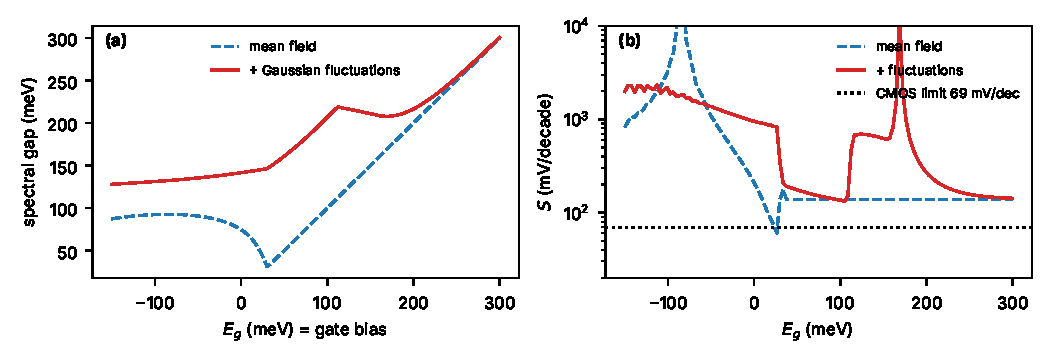
\includegraphics[width=\textwidth]{figs/fig3_switching.pdf}
\caption{Gap-switching transistor for MoSe$_2$/hBN/WSe$_2$ at 350~K. (a) Spectral gap versus $E_g$ (ideal gate), in mean field and with
Gaussian fluctuations. (b) Subthreshold swing, compared with the CMOS limit.}
\label{fig:switch}
\end{figure*}

\subsection{Machine-learning screen}
A bootstrap ensemble of gradient-boosted trees~\cite{Pedregosa2011} was trained on 3000 solver labels
$T_c=\min(T^*/2.2,\,T_{\rm BKT},\,\text{Eq.~(\ref{eq:ceiling})})$, with $0.01\le m_r\le1$, mass ratio 0.2--5,
$1.5\le\epsilon\le15$ and $0.3\le d\le10$~nm. On held-out data it reaches $R^2=0.87$ with a mean absolute error of 1.3~K, and 95\% of held-out points lie within the ensemble's own $\pm2\sigma$ predictive interval, so its uncertainty estimates are calibrated. Inverse design over $2\times10^5$ candidates, followed by verification with the full solver, gives at most
$\approx117$~K for $\epsilon\ge4.5$ and $\approx233$~K for $\epsilon\approx1.6$. One label of 3000 exceeds 350~K, at
$\epsilon=1.7$, $d=0.58$~nm and $E_g=-1.4$~eV, which is not a realistic device. The surrogate only interpolates the benchmarked model. It cannot discover mechanisms the model does not contain, so the inverse design bounds what this framework allows, not what all materials allow.

\section{Robustness, scope and limitations}
Several ingredients that could raise $T_c$ were treated optimistically: equal masses, $n_s=n$, an ideal gate in the bound, and
single-species screening. The main conclusions were tested against the most consequential approximations as follows.

\textit{Screening model.} Using the DQMC onset ($r_{s,c}\approx2.5$ at $d=a_B$~\cite{Neilson2014}) instead of the SS mean field gives
51~K for the MoSe$_2$/WSe$_2$ parameters of Ref.~\onlinecite{Zeng2020}. DQMC includes dynamic screening and vertex
corrections~\cite{Neilson2014}. Reaching 300~K there would require $r_{s,c}\le1.03$, less than half of both the SS and DQMC values. In the
most favourable hBN corner of the parameter box ($\epsilon=4.5$, $d=0.6$~nm), the ceiling is 146~K. It would reach 300~K only if the
true onset lay $\approx$30\% below the DQMC value. This is the margin by which the hBN conclusion depends on the screening physics.

\textit{Intralayer exchange.} It enters the compressibility $d\mu_x/dn$ and hence the gate response, which we bracket using the
exchange-dominated value of Ref.~\onlinecite{Zeng2020}. At 300~K the thermal compressibility $k_BT/n$ dominates both brackets. The
ceiling of Eq.~(\ref{eq:ceiling}) does not involve the compressibility.

\textit{Ta$_2$NiSe$_5$.} The thresholds depend on the mean-field decoupling; the excitonic share and the absence of superfluidity do not
(Sec.~III D).

\textit{Scope.} Only equilibrium, gate-driven operation is evaluated. The main limitations are: (i) static
mean field with Gaussian fluctuations, without vortex dynamics or vertex corrections beyond those tested in
Ref.~\onlinecite{Neilson2014}; (ii) no intralayer exchange in the continuum model, which changes the sign of the
exciton--exciton interaction compared with Ref.~\onlinecite{Zeng2020}; we use both as brackets; (iii) a 15--28\%
deviation from two Ta$_2$NiSe$_5$ numbers of Ref.~\onlinecite{Kaneko2013}. Its mean-field equations are given in supplementary material that was not used here, and two alternative Fock decouplings bracket the published values; and (iv) no transport, contact or circuit modelling. Non-equilibrium (optical) switching in Ta$_2$NiSe$_5$ and cryogenic
operation, where the CMOS limit falls to 15~mV/decade at 77~K, lie outside this screen.

\section{Conclusion}
Within benchmarked equilibrium models of 2D parabolic, Dirac and quasi-one-dimensional excitonic systems, gate-driven
excitonic-insulator switches do not beat CMOS in subthreshold swing or switching energy at 300--350~K. Tunnelling-based and
non-equilibrium (e.g.\ optically driven) excitonic switches are not ruled out by this analysis. Room-temperature pairing is
possible, but screening-limited 2D condensation is not. The steep switching that appears in mean field is an
artefact that Gaussian fluctuations remove. The design rule of Eq.~(\ref{eq:ceiling}) and the open code provide
a quantitative test for future excitonic device proposals.

\section*{Data availability}
All code, data and figure scripts are openly available at \url{https://github.com/masyhur-n/excitonic-insulator-sim}~\cite{repo} under the MIT license, and archived at Zenodo, doi:\href{https://doi.org/10.5281/zenodo.23684703}{10.5281/zenodo.23684703}~\cite{repo}.

\section*{Author declarations}
\noindent\textbf{Conflict of interest.} The author has no conflicts to disclose.\\
\textbf{Author contributions.} Nailah Masyhur: conceptualization, methodology, software, validation, formal analysis, writing (original draft, review and editing).\\
\textbf{Ethics approval.} Not applicable.\\
\textbf{Use of AI tools.} Code development, literature retrieval and drafting were assisted by an AI coding
assistant (Claude, Anthropic). The author directed the study, verified every result against the published
benchmarks listed in Table~\ref{tab:bench}, and takes full responsibility for the content.

\begin{acknowledgments}
The author thanks the authors of the benchmark studies whose published data made this verification possible.
\end{acknowledgments}

\bibliography{refs}

\end{document}
